\documentclass{article}
\usepackage[utf8]{inputenc}
\usepackage{subfig}

%References
\usepackage{natbib}
%IMPORTANT use https://www.citationmachine.net/ if you need to generate references!
% \citep{reference} creates Harvard Style references throughout

%Colors
\usepackage{xcolor}

\usepackage[protrusion=true,expansion]{microtype}

%Code Markup
\usepackage[outputdir=cache]{minted}
%Syntax Highlighting Style
\definecolor{bggray}{RGB}{40,40,40}
\newmintedfile[javacode]{java}{
	style=fruity,
	bgcolor=bggray,
	linenos,
	breaklines,
	tabsize=2,
	obeytabs
}

\newmintedfile[bashoutput]{text} {
	style=fruity,
	bgcolor=lightgray,
	breaklines,
	tabsize =2,
	obeytabs
}

%Page Margins and stuff
\usepackage{geometry}
 \geometry{
 a4paper,
 total={170mm,257mm},
 left=20mm,
 }

%Pictures
\usepackage{graphicx}
\graphicspath{ {./images/} }

%Move the title position
\usepackage{titling}

\setlength{\droptitle}{-8.5em} %Up, near the top but not too high

\title{Assignment 4 - CT2106 Object Oriented Programming}
\author{Daniel Hannon (19484286)}
\date{November 2020}

\begin{document}
	\maketitle
	\section{Overview}
	For this project we had to create a basic interface for a theoretical website called TravelIreland in which you have the ability to book bus tickets from three major bus companies:
	\begin{itemize}
		\item BusEireann
		\item Go Bus
		\item CityLink
	\end{itemize}
	As it is a consumer interface we imagine that the company class pulls trip data from the websites of the relative bus companies, consequently the only time bus ticket data can be edited is when a purchase is made and then the seats Available on the bus are reduced.\\
	As it would not make sense to make a completely new class for each travel company, they all inherit all their functions from an abstract class Company, which handles making bookings and keeps track of all the available bus journeys.\\
	The Trip class holds all relative data for a journey (Apart from the company name as that would not make sense if each company is a separate object).
	The Booking class is rather primitive as it holds the reference to the Trip, Quantity of seats, and the total cost of the booking (if Successful), everything within the booking class is evaluated by the Company class and TravelIreland class.\\
	TravelIreland is the class which implements the user interface itself, it communicates with the Company sub classes and then provides a very rudimentary interface so they can be utilized.
	\begin{figure}[h!]
		\centering
		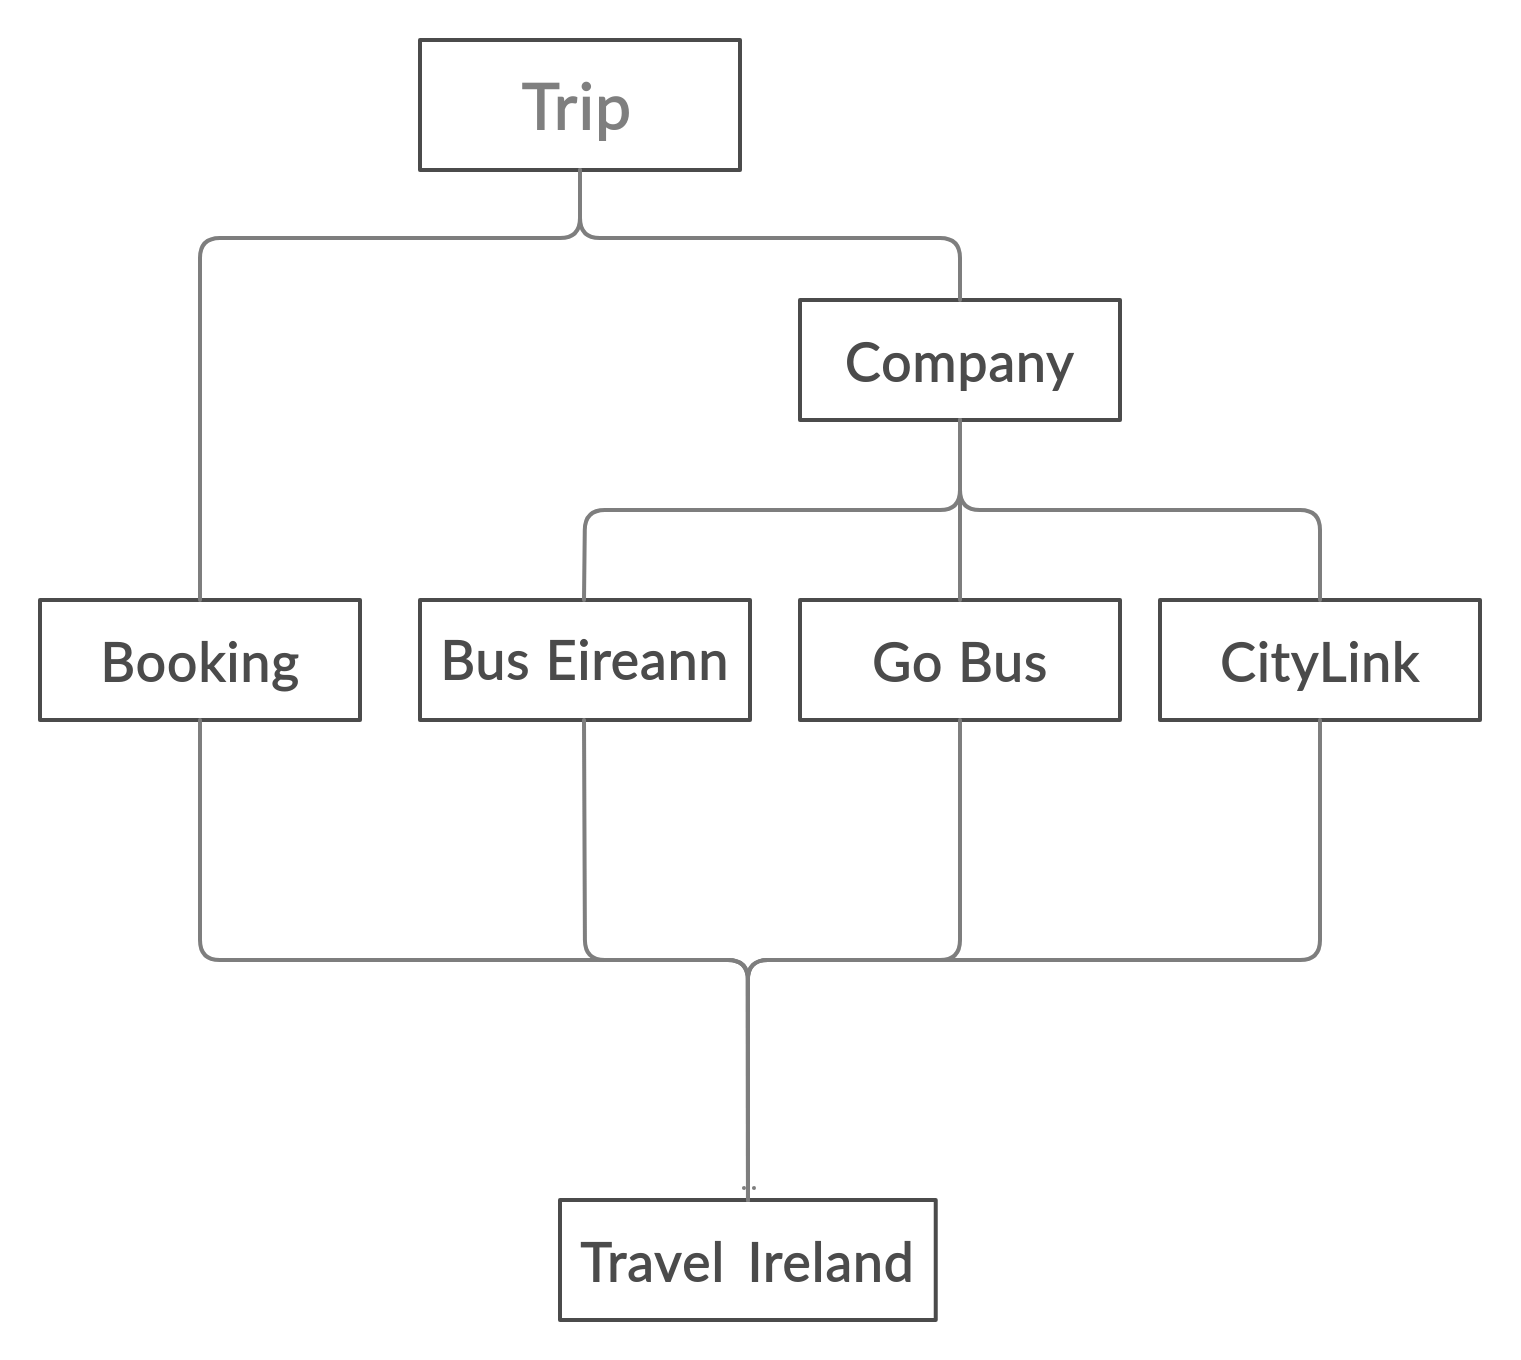
\includegraphics[width=0.8\textwidth]{hiearchy.png}
		\caption{Class Hiearchy}
	\end{figure}
	\section{Output}
	\bashoutput{output.txt}
	\section{Code}
	\subsection{Trip.java}
	\javacode{Trip.java}
	\subsection{Company.java}
	\javacode{Company.java}
	\subsection{Booking.java}
	\javacode{Booking.java}
	\subsection{BusEireann.java}
	\javacode{BusEireann.java}
	\subsection{CityLink.java}
	\javacode{CityLink.java}
	\subsection{GoBus.java}
	\javacode{GoBus.java}
	%Sets to Harvard Style and links the references file
	\bibliographystyle{agsm}
	\bibliography{references}
\end{document}
